\chapter{Introduction} \label{ch:Introduction}

This introductory chapter explains the notion of quantum information processing and why it might be useful.

\section{Information processing machines}

Information processing pervades our civilization.
Examples of information processing, essential to our way of life include communication, data storage and retrieval, and problem solving machines.
Digital information processing has become especially important since the invention of the vacuum tube, and later, the transistor.
We spend enormous effort and resources improving our information processing hardware: in 2013 Intel spent more than ten billion dollars on research and development \cite{Intel:earnings2013}.

\begin{figure}
\begin{centering}
\includegraphics[width=9cm]{mech_electronic_gates.pdf}
\par\end{centering}
\caption{Two physical implementations of logic elements. a) A mechanical OR gate. If either of the bottom rods is pushed, the output rod extends. If neither input rod is pushed, springs retract the output rod. b) An electronic NAND gate. If voltage is applied to both input wires then current flows freely through the transistors, bringing the output node to ground.}
\label{Fig:mechElectronicGates}
\end{figure}

\subsection{Information is physical}

A computer contains an array of physical elements, such as gears in a mechanical computer, or transistors in an electronic one.
The physical states of those elements stores information.
In the mechanical computer, the physical state is the rotational orientation of the gears, and in the electronic computer it is the current and voltage in the transistor.
Physical interactions between elements, causing them to change their state, achieves computation.
In a mechanical computer, sliding rods pushing on one another lead to the positions of a register of output rods which depend on the positions of the inputs.
In a solid state electronic computer, arrays of input voltages are transferred from memory circuits into the central processing unit (CPU) where they interact in logic circuits such as NAND or XOR gates to produce resulting output voltages.
Figure \ref{Fig:mechElectronicGates} illustrates two examples: a mechanical OR gate and an electronic NAND gate.
These examples are meant to emphasize the fundamentally physical nature of information processors.

\subsection{Classical physics limits information processing}


The above example computers, and in fact in any existing information processing device, ignore a great deal of information associated to the physical elements in the computer.
A particular state of a transistor implicitly includes an enormous set of possible microscopic states (``microstates'') of the individual electrons carrying the current.
This is illustrated in Fig.\,\ref{Fig:wireCurrent} where multiple microstates are shown for left flowing and right flowing macroscopic current states in a wire.
Information processing in the computer is insensitive to these microstates by construction.
Ignorance of this information is essential for the operation of a real machine: if the logical state of a transistor depended on the precise state of every electron, we would have to eliminate phonon scattering and operate at absolute zero temperature in order to have a usable machine.
In other words, ignorance of precise microscopic dynamics affords the computer robustness against real-world non-ideal effects.

On the other hand, it turns out that this ignorance restricts the computer to physical processes which obey classical physics.\footnote{A demonstration of \emph{why} this is the case will be given subsequently.}
At any point in the computation, the computer's state is described by independently specifying the state of each information storage element, \begin{eqnarray}
\ket{\textrm{computer}} &=& \ket{\textrm{state of }0^{th}\textrm{ element}} \ldots \ket{\textrm{state of }N-1^{th} \textrm{ element}} \nonumber \\
& \textrm{e.g.} & \ket{0}\ket{1}\ket{1}\ldots\ket{1}\ket{0}\ket{0} = \ket{011 \ldots 100} , \label{eq:classicalState} \end{eqnarray}
where 0 and 1 indicate the two possible states of a logic element.
Note that a system with $N$ bits requires $N$ 0's and 1's to specify its state.
While this representation may seem obvious and unavoidable, from a physical point of view it is somewhat limited.
We know that Nature fundamentally allows for physical states more complex than the one in Eq.\,(\ref{eq:classicalState}): quantum mechanics describes a physical state as a weighted superposition of states, such as $c_0 \ket{0} + c_1 \ket{1}$ where $ \left\{ c_i \right\} $ are complex numbers.
These superposition states are more complex than their classical counterparts, so use of only classical states in information processors limits their power.

\begin{figure}
\begin{centering}
\includegraphics[width=1.0\textwidth]{wireCurrent.pdf}
\par\end{centering}
\caption{A wire with two different macroscopic current states.(a) and (b) show three microscopic states corresponding respectively to rightward and leftward current. Note that in each microscopic state some electrons may be moving in a direction against the macroscopic current.}
\label{Fig:wireCurrent}
\end{figure}

Suppose we want to compute properties of $N$ quantum two level systems where each one interacts with its nearest neighbours, a so-called ``quantum spin chain'', as shown in Figure \ref{Fig:spinChain}\,a.
The system is described by $2^N - 1$ complex numbers $c_i$, \footnote{Normalization and the irrelevance of the global phase reduce the parameter count by 2 real numbers, or equivalently one complex number.} \begin{equation}
\ket{\textrm{spin chain}} = c_0 \ket{00 \ldots 00} + c_1 \ket{00 \ldots 01} + \cdots + c_{2^N} \ket{11 \ldots 11} \label{eq:quantumState}. \end{equation}
Note that each term in the sum corresponds to one complete classical state of the spin chain as in (\ref{eq:classicalState}).
The number of parameters needed to specify \emph{one particular} quantum state is proportional to the number of \emph{all possible} classical states.
Suppose each of the numbers $c_i$ is represented in a classical computer by an $m$ bit number.
Then, to represent a single state of the quantum system we need $m 2^N$ classical bits, so the size of the classical computer needed to simulate a quantum system grows exponentially in the size of the quantum system.
This illustrates one limitation of classical computers: they cannot efficiently store the information needed to represent quantum mechanical physics problems.

That classical computers cannot efficiently simulate quantum mechanics is not too surprising since we know that quantum states are more complex than classical ones.
However, classical computers seem to be limited even in their ability to solve abstract math and logic problems.
A famous example of this is the problem of finding the prime factors of an integer.
Although this problem has been known since ancient times, no polynomial time classical algorithm has ever been found.\footnote{A simple but slow algorithm for deciding whether a number is prime and finding its factors is attributed to Eratosthenes of Cyrene (c. 276\,BC - c. 195/194\,BC).}
The best modern algorithm, the general number field sieve \cite{Lenstra:sieve1993}, factors a $b$ bit number in time asymptotically proportional to \begin{equation}
\exp \left( \left( 1.9 + o(1) \right) (b\ln 2)^{1/3}(\ln (b\ln 2))^{2/3} \right) \end{equation}
in the limit of large $b$. Note the super-polynomial (but sub-exponential) scaling.

\subsection{Quantum Information}

\begin{figure}
\begin{centering}
\includegraphics[width=9cm]{spinChain.pdf}
\par\end{centering}
\caption{The physics of a quantum spin chain can be investigated by construction of a controllable and measurable analogue system. a) A physical spin chain. b) An array of two level systems engineered to match the physics of the spin chain.}
\label{Fig:spinChain}
\end{figure}

In the previous section, we showed that a quantum state cannot be efficiently stored on a classical computer.
This problem suggests its own solution: use an information processor in which the logic elements themselves are quantum mechanical.
A simple approach is to build an analogous system out of elements that are amenable to experimental control and measurement, as shown in Figure\,\ref{Fig:spinChain}\,b.
By engineering the analogue system to have the same physics (ie. same Hamiltonian) as the spin chain, we can infer properties of the spin chain from observations of the engineered system.
A realistic analogue system for the spin chain could be a chain of ions trapped in an optical lattice.
Existing technology allows for exquisite control and measurement of trapped ions.
Note that this idea of building an analogous system, or ``model'' that is amenable to precise engineering and measurement is not restricted to quantum systems.
Indeed, modeling has been used for architectural projects for centuries and is in some sense the oldest form of information processing.

The modeling approach works for systems in which the physics is simple enough that a controllable analogue system can be realized, but this will not always be possible.
It is difficult to imagine building a controllable analogue system for a high energy particle scattering problem.
For problems for which we cannot build models we need a more abstract approach.
Historically, we addressed this type of problem by constructing a mathematical model of the physics problem and solving the model with a numerical computer.
However, we already saw that a quantum state cannot be efficiently stored on a computer which uses classical physics.
Looking again at Figure \ref{Fig:spinChain}\,b, we can re-imagine the array of controllable two level quantum elements, originally conceived as a proxy for the spin chain, as a quantum bit register.
This suggests the notion of a general purpose abstract computer that uses quantum bits instead of classical ones.
Information would be processed by controlled interactions between quantum bits in the register.
We could engineer the interactions between two quantum elements such that they undergo specific transformations, akin to the classical logic gates used in normal computers such as XOR and NAND gates.
A quantum example is described by the following unitary matrix \begin{equation}
\begin{array}{c} \ket{00} \\ \ket{01} \\ \ket{10} \\ \ket{11} \end{array} \left[ \begin{array}{cccc} 1 & 0 & 0 & 0 \\ 0 & 1 & 0 & 0 \\ 0 & 0 & 0 & 1 \\ 0 & 0 & 1 & 0 \end{array} \right]. \label{eq:CNOT} \end{equation}
This operation is known as a ``controlled NOT'' or CNOT gate, because the state of the second bit inverts if the first bit is on (ie. in the $\ket{1}$ state).
This example shares with the classical cases the general idea of using controlled interactions to produce changes in the bits representing a logical computation.
Importantly, the quantum gate works on superposition states in addition to the usual classical states.
Operations like this could form a collection of quantum logic gates analogous to classical logic gates, and we can imagine a generic Turing-style computer based on transformation of quantum states through such gates.
Similarly to how the NOT and AND gates form a universal set of operations in classical computing, arbitrary single qubit controls along with the CNOT form a universal set for a quantum computer \cite{Barenco:gates1995}.

Amazingly, this kind of generic quantum information processor might be able to solve some types of abstract problems more efficiently than classical computers.
A famous algorithm for factoring prime numbers, Shor's algorithm \cite{Shor:algorithm1994}, runs on a quantum computer in a time that goes as a polynomial in the number of input digits.
This is an example of a case where a quantum computer solves an abstract problem more efficiently than a classical computer, and the practical application of prime factoring in cryptography is a strong driving force behind quantum information research.
It's important to note that the current lack of a known classical algorithm for prime factoring does not preclude the possibility that one will be found in the future.
It has not been proven that efficient factoring on a classical computer is impossible, and so the utility of quantum computers for abstract problem solving is not necessarily firmly established.
On the other hand, there is one known problem that quantum computers can solve faster than is possible on a classical computer: function inversion.
Given a function $f$, a set of possible inputs $\{x\}$ of length $N$, and an output $y$, the quantum ``Grover Search''\footnote{The Grover Search is some times described as a database lookup. The connection to function inversion comes by choosing $f$ such that $f(x)=\text{True}$ only when $x$ is the desired database entry. Note that, on a normal computer, \emph{structured} databases can be searched in constant time by using hash lookup or similar methods.} algorithm can find $x$ such that $f(x)=y$ in time proportional to $\sqrt{N}$.
Classically, the search time scales as $N$.
This square root speed-up for the quantum algorithm is less impressive than the near exponential speed-up associated to Shor's factoring algorithm, but is a strong indicator that quantum information processors are fundamentally more powerful than classical ones, at least for some types of problems.

\subsection{Summary}

Quantum information processors may be able to efficiently solve some problems that classical processors cannot. Quantum algorithms are known for prime factoring and function inversion.
The former represents a significant speed-up over known classical algorithms and seems very likely to indicate that quantum processors are significantly more powerful than classical ones.
The latter establishes that in at least one case quantum processors can solve problems faster than is fundamentally possible on a classical processor, although the speed-up is modest.
Quantum processors seem to be clearly superior to classical processors for quantum physics problems as they can more efficiently store the information needed to represent the state of the system being simulated.

Two types of quantum information processors were described. In the first type the processor is simply a model of a physics problem and is used to directly measure properties of the analogous system. In the second type an array of quantum elements are used as an information storage register and computations are done through physical interactions between them, just as in a normal computer.

\section{Quantum Bits}

To build a quantum computer, we need quantum mechanical logic elements that are controllable and measurable. As in the classical case, these elements could have any number of possible states, but analysis and construction is simplest in the case of two possible states. With homage to the term ``bit'' for a controllable two-state information storage element in classical computers, we refer to the quantum analogue as a \textbf{``qubit''}. In this section we explain why building usable qubits is hard. With that understanding we explain the requirements for a working quantum computer. Finally we discuss a few possible candidate physical systems for making qubits.

\subsection{Qubits are hard to make because quantum states are fragile} \label{sec:ch:introduction:coherence}

As discussed previously, classical computers are insensitive to many of the details of the physical processes taking place inside their bits.
As indicated in Figure \ref{Fig:wireCurrent}, the logical state of a transistor does not depend on the individual states of the electrons in the wire, but rather only on the average of those states.
The following states correspond to upward current \begin{equation}
\left\lbrace \ket{\uparrow \uparrow \uparrow}, \ket{\downarrow \uparrow \uparrow}, \ket{\uparrow \downarrow \uparrow}, \ket{\uparrow \uparrow \downarrow} \right\rbrace \end{equation}
and the following correspond to downward current \begin{equation}
\left\lbrace \ket{\downarrow \downarrow \downarrow}, \ket{\uparrow \downarrow \downarrow}, \ket{\downarrow \uparrow \downarrow}, \ket{\downarrow \downarrow \uparrow} \right\rbrace \end{equation}
where $\uparrow$($\downarrow$) indicates a single electron carrying current upward(downward).
The computer's ignorance of the individual electron states means that if the system undergoes a transition \begin{equation}
\ket{\uparrow \uparrow \uparrow} \rightarrow \ket{\downarrow \uparrow \uparrow}, \label{eq:allowedTransition} \end{equation}
then the state of the transistor, and thus the logical state of the computer, does not change.
For classical computers this is an essential feature: if the computer's state depended on such microscopic processes we would have to completely eliminate all scattering processes in the wires, a seemingly impossible task.
By remaining insensitive to these processes the classical computer can operate at finite temperatures with imperfect materials, etc.
Now, it turns out that ignorance of these processes is also what makes the machine classical instead of quantum mechanical.
To see why, suppose we have a pair of transistors in an initial quantum state \begin{equation}
\ket{\textrm{transistors}} = \ket{\uparrow \uparrow \uparrow}\ket{\uparrow \downarrow \downarrow} + \ket{\downarrow \downarrow \downarrow}\ket{\uparrow \uparrow \uparrow} \equiv \ket{1}\ket{0} + \ket{0}\ket{1} \end{equation}
where $\ket{1}$ means upward current and $\ket{0}$ means downward current. Now suppose the first transistor suffers the transition given in (\ref{eq:allowedTransition}). The resulting transition for the computer is \begin{eqnarray}
\textrm{physical:} \quad \ket{\uparrow \uparrow \uparrow}\ket{\uparrow \downarrow \downarrow} + \ket{\downarrow \downarrow \downarrow}\ket{\uparrow \uparrow \uparrow} & \rightarrow & \ket{\downarrow \uparrow \uparrow}\ket{\uparrow \downarrow \downarrow} + \ket{\downarrow \downarrow \downarrow}\ket{\uparrow \uparrow \uparrow} \nonumber \\
\textrm{logical:} \quad \ket{1}\ket{0} + \ket{0}\ket{1} & \rightarrow & \ket{1}\ket{0} + \ket{0}\ket{1}. \end{eqnarray}
The logical state does not change, so it appears that nothing important has happened.
However, the electron state change cannot happen in isolation.
If the electron state changes, it must be due to interaction with something else.
Suppose the electron state change coincides with creation of a phonon in the wire.
Adding the phonon state to our representation, we re-write the electron state change process as \begin{eqnarray}
\ket{\text{computer}} & \rightarrow & \ket{\text{computer}'} \nonumber \\
\text{physical:}\quad \ket{\uparrow \uparrow \uparrow}\ket{\uparrow \downarrow \downarrow}\ket{0} + \ket{\downarrow \downarrow \downarrow}\ket{\uparrow \uparrow \uparrow}\ket{0} & \rightarrow & \ket{\downarrow \uparrow \uparrow}\ket{\uparrow \downarrow \downarrow}\ket{1} + \ket{\downarrow \downarrow \downarrow}\ket{\uparrow \uparrow \uparrow}\ket{0} \nonumber \\
\text{logical:} \quad \ket{1}\ket{0}\ket{0} + \ket{0}\ket{1}\ket{0} & \rightarrow & \ket{1}\ket{0}\ket{1} + \ket{0}\ket{1}\ket{0} \label{eq:scattering} \end{eqnarray}
where here the third ket being $\ket{0}$($\ket{1}$) represents the absence(presence) of the phonon, and the prime indicates the computer's state after the transition.
The information carried by the state of the phonon is not available to the computer, so to understand what information is still carried by the computer we must re-express the state without the phonon .
On the left hand side of Eq.\,(\ref{eq:scattering}) the phonon is always in state $\ket{0}$, so the information available to the computer is easily written by dropping the phonon part \begin{equation}
\ket{\text{computer}} = \ket{1}\ket{0} + \ket{0}\ket{1} \end{equation}
The right hand side of Eq.\,(\ref{eq:scattering}) includes terms where the phonon state is not always the same.
It turns out that in this case, the state takes on a statistical nature \footnote{This can be shown rigorously using the density matrix formalism.} \begin{equation}
\ket{\text{computer}'} = \left\{ \begin{array}{c}
\ket{0}\ket{1} \quad \text{probability}= 1/2 \\
\ket{1}\ket{0} \quad \text{probability}= 1/2 \end{array} \right. . \end{equation}
The state after the phonon scattering event, $\ket{\text{computer}'}$, is a statistical mix of either $\ket{10}$ \emph{or} $\ket{01}$ with no quantum superposition.
You can think of this as a collapsed wave function that occurs after the phonon measures the state of the first electron.
With the quantum superposition in the computer state now gone, the computer's function is limited to processes described in classical physics.

% Here follows an explanation using the density matrix. John commented that this is too mathy and avoids physical reasoning, so I've commented it out for future reference.
%In the case that our machine's operation does not depend on the state of the phonons, the information available to that machine cannot be represented as a quantum state vector. Instead, it must be expressed as a density matrix. The density matrix of the system prior to the scattering event (left side of (\ref{eq:scattering})) is \begin{eqnarray}
%\rho &=& \left[ \left( \ket{\uparrow \uparrow \uparrow}\ket{\uparrow \downarrow \downarrow}\bra{\uparrow \uparrow \uparrow}\bra{\uparrow \downarrow \downarrow} \right) + \left( \ket{\downarrow \downarrow \downarrow}\ket{\uparrow \uparrow \uparrow}\bra{\downarrow \downarrow \downarrow}\bra{\uparrow \uparrow \uparrow} \right) \right. \nonumber \\
%& & \left. + \left( \ket{\uparrow \uparrow \uparrow}\ket{\uparrow \downarrow \downarrow} \bra{\downarrow \downarrow \downarrow}\bra{\uparrow \uparrow \uparrow} \right) + \left( \ket{\downarrow \downarrow \downarrow}\ket{\uparrow \uparrow \uparrow}\bra{\uparrow \uparrow \uparrow}\bra{\uparrow \downarrow \downarrow} \right) \right] \nonumber \\
%& & \otimes \ket{0}\bra{0} \nonumber \\
%&=& \left[ \ket{10}\bra{10} + \ket{01}\bra{01} + \ket{10}\bra{01} + \ket{01}\bra{10} \right] \otimes \ket{0}\bra{0} \label{eq:coherentStateWithPhonon} \end{eqnarray}
%The off diagonal terms like $\ket{01}\bra{10}$ in (\ref{eq:coherentStateWithPhonon}) represent the ability for the state to undergo quantum interference. The density matrix for the system after the scattering event (right side of (\ref{eq:scattering})) is \begin{eqnarray}
%\rho ' &=& \ket{10}\bra{10}\otimes\ket{1}\bra{1} + \ket{01}\bra{01}\otimes\ket{0}\bra{0} \nonumber \\
%& & + \ket{10}\bra{01}\otimes\ket{1}\bra{0} + \ket{01}\bra{10}\otimes\ket{0}\bra{1} \end{eqnarray}
%To compute the available information in the computer in ignorance of the state of the phonons, we take the trace of $\rho$ over the phonon state, resulting in \begin{eqnarray}
%\rho &=& \ket{10}\bra{10} + \ket{01}\bra{01} + \ket{10}\bra{01} + \ket{01}\bra{10} \label{eq:coherentState} \\
%\rho' &=& \ket{10}\bra{10} + \ket{01}\bra{01} \label{eq:decoheredState} \end{eqnarray}
%which can be found by keeping only terms for which the phonon bra and ket states are the same. The density matrix in (\ref{eq:decoheredState}) is missing the off-diagonal terms from (\ref{eq:coherentState}). In fact, the density matrix $\rho'$ in (\ref{eq:decoheredState}) represents a probabilistic mix of either $\ket{10}$ \emph{or} $\ket{01}$ with no quantum superposition. You can think of this as a collapsed wave function that occurs after the phonon measures the state of the first electron. With the quantum superposition in the computer state now gone its function is limited to processes described in classical physics.

It only required \emph{one} electron state change in a phonon scattering event to cause the \emph{complete} destruction of the computer state's quantum superposition.
In a real transistor, with orders of magnitude more electrons, single scattering processes like the one illustrated here are overwhelmingly likely to occur with extremely high frequency.
This explains why quantum coherence is so fragile and illustrates why normal computers are classical.\footnote{In fact, what we have illustrated here may be the essence of why we do not observe quantum interference in common experience.}
The phenomenon illustrated here, by which quantum superposition of a subsystem is lost when it interacts with other degrees of freedom, is known as ``decoherence''.
The surrounding degrees of freedom are called the ``environment'', and when some of the information of the subsystem has leaked into the environment, the subsystem and environment are said to be ``entangled''.
Identification of processes causing decoherence and elimination of those processes is one of the crucial challenges of experimental quantum information.

Decoherence in qubits is typically characterized by the rates of two types of processes.
The first process is decay from $\ket{1}$ to $\ket{0}$ accompanied by absorption of a quantum of energy from the qubit by something in the surrounding environment.
This process frequently occurs with constant probability per unit time and can therefore be described by an exponential time constant $T_1$.
The second process is randomization of the relative phase between $\ket{0}$ and $\ket{1}$, caused by fluctuations in the energy difference between those two states.
This is typically characterized by a time constant $T_2$, although in many systems the noise responsible for this process is correlated in time, so the decoherence does not go exponentially and must be described by a more complex function of time, such as $\exp \left[ -t/T_{\phi_1} - (t/T_{\phi_2})^2 - \cdots \right]$.

\subsection{Requirements for a quantum computer}

The requirements for a working quantum computer are summarized in the ``DiVencenzo criteria'' for a set of usable qubits:
\begin{enumerate}
\item Reliable qubit state preparation
\item Low qubit decoherence
\item Accurate quantum logic operations for single qubits and between pairs of qubits
\item Accurate measurement of the qubit states
\end{enumerate}
Items 2, 3, and 4 are interrelated and warrant discussion.
Low decoherence is not really a meaningful criterion by itself.
If it were required that qubits maintain coherence for the entire duration of a quantum computation, the task would appear hopeless: in order to have a fixed system error rate, the coherence of each qubit would have to scale exponentially with the number of qubits.
However it is theoretically possible to use qubits in an algorithm lasting much longer than the their coherence times by using error correction.
With quantum error correction, the important figure of merit is the ratio of the qubit coherence times to the time needed for an error correction cycle.
Error correction typically involves several single and two qubit logic gates followed by projective measurement of a subset of the qubits, and succeeds in preserving the logical state of the computer if those operations and measurements are done with high enough accuracy and large enough system size.
Therefore, in order to actually run a quantum computer, we need to be able to do only a \emph{few} logic operations with high accuracy in times short compared to the qubit coherence times.
Similarly the projective measurement must be done in a time short compared to the qubit coherence times, and must be done with high accuracy.
The precise meaning of ``high accuracy'' will be discussed later.

From the previous section, it is clear that there is an intrinsic tension between accurate control for logic operations and qubit coherence.
By construction, the hardware coupled to the qubits to control their states introduces decoherence channels.
The same is true for the apparatus used to measure the qubits' states.
Navigating this tension is the main challenge of experimental quantum information.

\subsection{Candidate systems for qubits}

\begin{figure}
\begin{centering}
\includegraphics[width=9cm]{qubitTypes.pdf}
\par\end{centering}
\caption{Qubit implementations. a) Electrons embedded in a semiconductor are used as qubits through their spin degree of freedom. This image shows a pair of ``double quantum dot'' qubits. In each one, two electrons are used to implement a single logical qubit. Note the large number of control wires. The image was taken from the website of Amir Yacoby at Harvard. b) Ions trapped in a linear ``Paul trap''. Blue arrows indicate axes through which laser light is brought into the trap to control the qubit states. State measurement is done through a state dependent fluorescent technique and the outgoing light is collected by a CCD camera. The image was taken from the website of Rainer Blatt at Innsbruck.}
\label{Fig:qubitTypes}
\end{figure}

In this section we describe two real qubit implementations and discuss the challenges involved in using them to build a quantum computer.

\subsubsection{Electron spin}
Single electron spins have the natural advantage that they are two level systems by nature and can be controlled via their magnetic dipole moment.
Typical experiments work with electrons embedded in semiconductors, as shown in Fig.\,\ref{Fig:qubitTypes}\,a.
Metal electrodes formed lithographically on the surface of the semiconductor produce electromagnetic fields which contain and control the qubit states.
A challenge with electron spin qubits is that the parameters of the qubit depend on microscopic properties of the semiconductor crystal in which the electrons are embedded.
In engineering parameters of the quantum computer, we are constrained not only by the general physics of electron spins in a crystal, but also by what materials can actually be realized.
The problem of growing a material compatible with high accuracy two qubit logic gates is a subject of ongoing research.

Another challenge comes from the weak and short range nature of the dipole interaction, which requires that the electrons be kept very close together in order to perform two-qubit logic operations.
This presents a challenge for bringing control wires into the system; the area needed by the control wires in Fig.\,\ref{Fig:qubitTypes}\,a is large compared to the area of the qubits, which makes scaling to a large computer system difficult.

\subsubsection{Trapped ions}
Another very successful qubit system is a single atom.
For each atom, two electron orbital states are chosen as the logic levels $\ket{0}$ and $\ket{1}$.
This system has the advantage of relatively long intrinsic coherence times, as it is possible to choose electron levels for which conservation rules suppress spontaneous decay, as used in atomic clocks.

The single atom qubit suffers several challenges.
First, their microscopic size and gaseous state requires that they be ionized and held in space by RF or optical laser fields, as shown in Fig.\,\ref{Fig:qubitTypes}\,b \cite{Blatt:review2008}.
Second, to remove scattering processes between the trapped ion and atmospheric molecules which would destroy the ions' quantum coherence, experiments must be done in ultra high vacuum.
Third, the use of electron levels for which coupling to the electromagnetic field is suppressed necessitates the use of strong lasers to induce qubit state transitions.
High power stable lasers are not part of a large consumer market, so ion trap labs must expend a great deal of time and effort to build lasers suitable for quantum computing.
Finally, the coupling between the ions' logical states is intrinsically weak.
While the ions, being charged, interact through the monopole Coulomb interaction, that interaction does not depend on the orbital state of the electrons.
When an ion's electron changes orbital state, that ion's electromagnetic field changes only in higher multipole moments.
With a single electron charge and subatomic displacement scales, the direct ion-ion interactions is too weak to be useful.

This last difficulty has been overcome in practice by using laser pulses to transduce the electron states to a vibrational motion of the ion within the trap, which then couples to the vibrational motion of other ions via the Coulomb force \cite{Sorensen:ions1999}.
This strategy has been used to implement high accuracy two qubit logic gates \cite{Benhelm:towardFaultTolerance2008}.

The challenges found in the examples presented here can all be attributed fundamentally to the fact that the qubits are based on naturally occurring microscopic objects. Because of this, the parameters of the qubit system come from Nature rather than from our own design.
In the next section we introduce a type of qubit that solves this problem.


\section{Superconducting Qubits}

Microscopic quantum objects like an electron spin or single atom constrain the design of an information processor because the processor inherits restrictions imposed by the fundamental physics of the microscopic system. Alternatively, we can start with an engineered system, like an electronic transistor, and try to make it quantum. This approach avoids restrictions imposed by e.g. the values of fundamental constants on Nature.

\begin{figure}
\begin{centering}
\includegraphics[width=9cm]{superconductingQubits.pdf}
\par\end{centering}
\caption{Superconducting qubits. a) A parallel $LC$ circuit.
b) The excitation spectrum of the system constructed with normal metal includes a dense set of electron excitations.
These excitations interact with the circuit resonance and destroy quantum coherence.
c) If the circuit is constructed with superconducting metal, the electron states vanish, leaving the circuit mode isolated and able to exhibit quantum coherence.
d) The quantized mode of the $LC$ circuit.
The quadratic potential leads to equally spaced energy levels.
e) A Josephson junction is formed by a thin insulating barrier interrupting two superconducting electrodes.
The circuit model symbol for a Josephson junction is a cross.
f) Replacing the linear inductor with a Josephson junction creates an anharmonic oscillator.
g) The anharmonicity leads to unequally spaced energy levels.
The lowest two levels can be used as a qubit.}
\label{Fig:superconductingQubits}
\end{figure}

\subsection{Quantum modes with engineered parameters}

As discussed in section \ref{sec:ch:introduction:coherence}, the current and voltage state of a normal metal wire is not quantum because information is lost in internal scattering processes. To get rid of scattering we could use a superconductor. In a superconductor there is an energy gap above the ground state within which there are no available system excitations. As long as the superconductor is not subject to stimulation by energy near or exceeding this gap, the individual electrons remain in the superconducting condensate ground state. Therefore, processes like the one illustrated in Eq.\,\ref{eq:allowedTransition} cannot occur and it should be possible to find quantum coherence in the macroscopic current.

Consider an LC circuit as shown in Fig.\,\ref{Fig:superconductingQubits}\,a.
From Kirchoff's laws we find the equations of motion for the charge $Q$ on the capacitor and flux $\Phi$ in the inductor, \begin{equation}
\dot{Q} = - \Phi/L \qquad \dot{\Phi} = Q/C . \label{eq:classicalOscillatorHamiltonsEquations} \end{equation}
Solving these gives charge and flux oscillating at a frequency $\omega_0 = 1/\sqrt{LC}$.
This mode corresponds to collective motion of the individual electrons in the metal.
In a normal metal circuit there are many other degrees of freedom, such as the individual electron and phonon states.
These degrees of freedom undergo constant scattering processes which prevent the macroscopic charge and flux oscillation mode from exhibiting quantum behavior, as illustrated in Fig.\,\ref{Fig:superconductingQubits}\,b.
However, if the electrons are all in the superconducting ground state, then there are no spurious microscopic processes and equations (\ref{eq:classicalOscillatorHamiltonsEquations}) represent the \emph{only} dynamics in the system, as illustrated in Fig.\,\ref{Fig:superconductingQubits}\,c.
The absence of interaction with environmental degrees of freedom preserves the quantum coherence of the resonance mode, as explained in section \ref{sec:ch:introduction:coherence}.
In that case we can represent the mode by a Hamiltonian for just the resonance degree of freedom, \begin{equation}
\hat{H} = \frac{\hat{Q}^2}{2C} + \frac{\hat{\Phi}^2}{2L} , \end{equation}
which, for the harmonic case, has a set of states spaced in frequency by $\omega_0=1/\sqrt{LC}$, as shown in Fig.\,\ref{Fig:superconductingQubits}\,d.
This is a remarkable idea: the collective motion of electrons in a superconducting resonant circuit should have quantum levels.
This is surprising if we are used to quantum mechanics applying only to microscopic objects.

\subsection{Superconducting circuits allow qubit engineering}

The resonant system has many energy levels, and the bottom two levels could be used as a qubit.
As the level spacing is determined by artificially engineered components $L$ and $C$, we are at liberty to \emph{engineer} our qubit's frequency for our convenience.
Furthermore, as shown in Appendix \ref{appendix:qubitTheory}, it turns out that if we connect two circuits through a capacitor $C_g$, the coupling energy $g$ normalized to their frequencies is \begin{equation}
\frac{g}{\hbar \sqrt{\omega_1 \omega_2}} = \frac{1}{2} \frac{C_g}{\sqrt{C_1 C_2}}. \end{equation}
Here $\omega_{1,2}$ are the frequencies of the two circuits, and $C_{1,2}$ are their self capacitances.
The right hand side depends on no constants of Nature.\footnote{Of course, realizable capacitances are limited by the value of the electrical permittivity $\epsilon_0$. Still, realizable capacitance ranges over several orders of magnitude.}
As capacitors and inductors are routinely built with values ranging over many orders of magnitude, superconducting circuits provide a great deal of flexibility in designing a quantum computer.
This should be contrasted against the situation with microscopic single particle qubits where intrinsic coupling strengths are constrained by constants of Nature.

\subsection{Non-linearity: Josephson junction}

The linear oscillator discussed above cannot easily be used as a qubit.
In the harmonic system, driving the system into states which can carry out information processing requires measurement of complex quantities such as parity.
One way to see this is to realize that an arbitrary array of linearly coupled harmonic oscillators is an analytically solvable problem.
Classical computers use the nonlinear physics of the transistor to effect information processing.
However, transistor physics is incompatible with the superconducting state.
To build a quantum computer with superconductors we need a nonlinear superconducting element.
Miraculously, there exists such an element: the Josephson tunnel junction \cite{Josephson:junction1962}.
A Josephson junction is a thin insulating barrier interrupting a superconducting wire, as shown in Fig.\,\ref{Fig:superconductingQubits}\,e.
The presence of the insulating barrier allows the superconducting condensate phases of the two electrodes to differ.
We denote the phase difference as $\delta$.
Current and voltage at the junction are related to $\delta$ through the Josephson relations \cite{Josephson:junction1962} \begin{equation}
I = I_c \sin(\delta) \qquad V = \frac{\Phi_0}{2\pi}\dot{\delta} \label{eq:josephsonRelations} . \end{equation}
Here $I_c$ is the ``critical current'' of the junction and $\Phi_0 = 2\times 10^{-15}\,\textrm{Weber}$ is the flux quantum.
The critical current is related to the normal state resistance of the junction $R_n$ and the superconducting gap $\Delta$ by the Ambegaokar-Baratoff relation \begin{equation}
I_c = \frac{\pi \Delta}{2 e R_n}. \end{equation}
Introducing the flux $\Phi \equiv \int V(t)\,dt$ and integrating the second Josephson relation gives a relationship between $\Phi$ and $\delta$, \begin{equation}
\delta = 2 \pi \Phi / \Phi_0 . \label{eq:deltaVsphi} \end{equation}
Using Eq.\,(\ref{eq:deltaVsphi}), the Josephson relations become \begin{equation}
I = I_c \sin \left( 2\pi \Phi / \Phi_0 \right) \qquad V = \dot{\Phi} . \label{eq:josephsonRelations_flux} \end{equation}
To lowest order in $\Phi/\Phi_0$, the first of equations (\ref{eq:josephsonRelations_flux}) is \begin{equation}
\Phi \approx \frac{\Phi_0}{2\pi I_c} \, I . \label{eq:ch:introduction:PhiVsIApprox} \end{equation}
From the usual relation $\Phi = LI$, Eq.\,(\ref{eq:ch:introduction:PhiVsIApprox}) gives a small signal inductance for the junction $L_{J_0} \equiv \Phi_0 / 2 \pi I_c$.
For arbitrary signals we compute the differential inductance \begin{equation}
L_J \equiv V / \dot{I} = \frac{\dot{\Phi}}{2 \pi I_c \dot{\Phi} \cos \left( 2 \pi \Phi / \Phi_0 \right) / \Phi_0} = \frac{L_{J_0}}{\cos(\delta)} = \frac{L_{J_0}}{\sqrt{1 - \left( I / I_c \right)^2}} . \end{equation}
This relation shows that the Josephson junction is a nonlinear inductor, with inductance diverging to infinity as the current through the junction approaches $I_c$.

Integrating the work done on this nonlinear inductor gives an expression for the energy stored, \begin{equation}
E = \int IV dt = \int I_c \sin(\delta) \frac{\Phi_0}{2\pi}\dot{\delta}dt = -E_J \cos(\delta) = -E_J \cos \left( 2 \pi \Phi / \Phi_0 \right) \label{eq:junctionEnergy} \end{equation}
where $E_J \equiv \Phi_0 I_c / 2\pi$.
Replacing the linear inductor with a Josephson junction, we get the circuit shown in Fig.\,\ref{Fig:superconductingQubits}\,f, where the potential energy is now a cosine as shown in Fig.\,\ref{Fig:superconductingQubits}\,g.
In the cosine potential, the circuit oscillation frequency decreases with increasing amplitude.
This is easily understood as a decrease in the oscillation frequency $\omega = 1/\sqrt{LC}$ as the junction inductance $L$ increases with increasing current.

We now turn to the quantum mechanics of the nonlinear circuit.
With the cosine potential from the junction, the circuit Hamiltonian becomes \begin{equation}
\hat{H} = \frac{\hat{Q}^2}{2C} - E_J \cos(\hat{\delta}) = \frac{\hat{Q}^2}{2C} - E_J \cos(2 \pi \hat{\Phi}/\Phi_0). \end{equation}
The energy levels of this Hamiltonian are shown in Fig.\,\ref{Fig:superconductingQubits}\,g.
Note that, unlike the case of the linear inductor with the parabolic potential, the energy levels in the junction circuit are unequally spaced.
This makes it possible, by bringing two qubits' $\ket{0}\rightarrow \ket{1}$ transitions on resonance with one another, to effect useful information processing on pairs of circuits.
Therefore, the circuit shown in Fig.\,\ref{Fig:superconductingQubits}\,f can be used as a qubit.

\subsection{Advantages of superconducting qubits}

We already saw that superconducting circuits allow enormous flexibility in constructing the parameters for a quantum computer because the single qubit parameters and two-qubit couplings are determined by engineered design rather than by constants of Nature. Here we list some other important advantages.

\begin{itemize}
\item In order for a superconducting circuit to be used as a qubit, the spacing between its energy levels must be larger than the surrounding thermal energy scale. In other words, we need $\hbar \omega_0 \gg k_b T$. Conventional dilution refrigerators attain temperatures of ten to a few tens of mK. At $T=20\textrm{mK}$ we would need a frequency of 3\,GHz to keep the thermal occupation of the qubit's excited state below a part in one thousand. This microwave frequency range is readily accessible with commercial electronic hardware. High quality tunable microwave sources available for a few tens of thousands of dollars are stable enough for use with superconducting logic gates with errors less than a part in one thousand. The commercial support in the frequency range needed for superconducting qubits is a major advantage.

\item Due to the prevalence of CMOS technology, fabrication of electrical circuits is an extremely well developed industry. Even the most complicated superconducting qubit chips requiring seven layers of lithography can be made in a couple of days in an academic clean-room facility. Construction by photo and e-beam lithography also directly enables scaling to larger system sizes.

\item Test and measurement instrumentation for electronics is extremely well developed. The dynamic range of standard microwave equipment such as spectrum analyzers, sources, and even arbitrary waveform generators allows the researcher to easily control and debug the superconducting qubit system. To give a sense of scale, microwave frequency DAC chips with 14 bit (42 dB) resolution are commercially available.

\item The connectivity of a superconducting qubit network is subject only to the constraints of on-chip wiring. This allows for very complex connectivity, as illustrated by the DWave ``chimera graph'' in which some qubits are connected to up to eight other qubits \cite{Boixo:annealing100Qubits2013}.
\end{itemize}

\subsection{Disadvantages - outstanding challenges}

To complete the picture of superconducting qubits within the field of quantum computation, we list some of their disadvantages and outstanding challenges.

\begin{itemize}
\item The large size of superconducting qubits makes them susceptible to decoherence processes.
A single superconducting qubit may interact with many material defects on the metal surfaces, and inside the tunnel junction or capacitor gaps.
These processes have limited the coherence time of the phase qubit to $\sim 1\,\mu\text{s}$, and have rendered the charge qubit essentially unusable.

\item Superconducting qubits are not true 2-level systems.
The one dimensional potentials admit higher quantum levels which can be inadvertently populated during information processing.
Unwanted transitions to higher levels devastate information processing protocols, as the qubit leaves the expected space of states.
In some types of qubits, such as the flux and fluxonium qubits, the nonlinearity from the Josephson junction can be large enough that this is not a problem in practice.
However, in the transmon qubit \cite{Koch:transmon2007}, the $\ket{1}\rightarrow\ket{2}$ transition frequency differs from the $\ket{0}\rightarrow\ket{1}$ transition frequency by only 3 to 4\%.
This small nonlinearity places restrictions on the speed of quantum gates in transmon qubits, and complicates two-qubit interactions, as the unwanted $\ket{1}\rightarrow\ket{2}$ transition must be carefully avoided.

\item Superconducting qubits rely on the disappearance of scattering states in the superconducting state to maintain coherence.
This requires the devices be placed in a cryostat to keep the temperature below the critical temperature of the superconducting material.
Furthermore, the temperature must be such that $k_b T << \hbar \omega_{\text{qubit}}$.
With $\omega_{\text{qubit}}/2\pi \approx 4\,\text{GHz}\text{ to }10\,\text{GHz}$, this requires $T\lesssim 200\,\text{mK}$.
Such low temperatures require Helium dilution refrigerators, limiting the available space for the experiment and accessibility for control wiring.
The Helium dilution process relies on $^3 \text{He}$, which is rare and expensive.

\item Unlike qubits based on individual microscopic particles, the individual qubits in a large array of superconducting qubits are not all guaranteed to be identical.
Imperfections in the fabrication process of superconducting qubits leads to devices with different inductance and capacitance.
In systems where the oscillation frequency of the qubits cannot be tuned \emph{in situ}, this poses a serious challenge.
Qubits with tunable frequency largely mitigate this problem.
\end{itemize}

\section{Fault tolerance}

Even in the superconducting state, the qubit oscillating mode interacts with external degrees of freedom.
Charged quasiparticle excitations of the superconducting condensate can absorb quanta of energy from the qubit as they tunnel across the Josephson junction.
Charged material defects, in the junction or in the qubit capacitors, feel the oscillating electric field of the qubit mode and can also absorb energy.
Superconducting qubits are macroscopically large, so we do not expect that these and other decoherence processes can ever be completely eliminated.

Suppose we were to try to build a quantum computer which would work in the presence of decoherence processes.
As illustrated in section \ref{sec:ch:introduction:coherence}, a single interaction even between the qubit and an external mode can destroy the coherence of the quantum state.
Therefore, we would have to reduce the rate of such events to the level that the probability of a single event is of order 1 or less over the entire duration of the quantum algorithm.
The numbers are not favorable.
The most efficient useful algorithms require a number of qubits $n_{\text{qubits}}\approx 100$ and a number of gates $N_{\text{gates}}\propto N_{\text{qubits}}^3$.
The probability that a single qubit with coherence time $T_{\text{coh}}$ does not suffer a decoherence event is \footnote{The discussion here pertains only to decoherence processes which are described as an exponential decay, ie. with a rate. Not all decoherence processes produce exponential decay, most notably the low frequency flux noise responsible for phase decoherence in superconducting qubits. Still, the essence of the present discussion remains intact.}
 \begin{equation}
P = e^{-t/T_{\text{coh}}} .\end{equation}
Denoting the total algorithm time as $T_{\text{alg}}$, the number of gates in the algorithm $N_{\text{gates}}$, and the time of a single gate as $T_{\text{gate}}$, we find \begin{equation}
\ln P = -\frac{T_{\text{alg}}}{T_{\text{coh}}} = -N_{\text{gates}} \frac{T_{\text{gate}}}{T_{\text{coh}}} . \end{equation}
To get a reasonable probability of the qubit remaining coherent, say $P=1/2$, the coherence time to gate time ratio is \begin{equation}
\frac{T_{\text{coh}}}{T_{\text{gate}}} = -\frac{N_{\text{gates}}}{\ln P} \gtrsim 10^6 \end{equation}
where in the last step we assumed $N_{\text{qubits}}=100$ and $N_{\text{gates}}=N_{\text{qubits}}^3$.
Current state of the art qubit systems achieve $T_{\text{coh}}/T_{\text{gate}} \approx 300$ \cite{Barends:gates2014}.
Improving coherence by a factor of $10^4$ is a daunting task, but even more importantly, qubit gate errors can also come from the control pulses used to generate the gates.
This means that the error per gate from the control pulses must also be at the $10^{-6}$ level.
Current state of the art for two qubit gates is a bit worse than $10^{-3}$ \cite{Barends:gates2014}.

So far, we have discussed the error rate for a single qubit.
However, the quantum computation is spoiled if \emph{any} qubit suffers an error.
This lowers the necessary error rate by a factor of $N_{\text{qubits}}$, which is at least a few hundred for useful algorithms.
This puts the required error rate per qubit gate at $10^{-8}$, an apparently impossibly low number.
From this discussion we see that brute force improvement of qubit errors is not a viable strategy for building a quantum computer.
Fortunately, there is better way.

It turns out that quantum information can be processed in way that tolerates errors.
The details of how this works are beyond the scope of this thesis, but we explain the basic idea here.
First, consider the state of a transistor in a classical computer.
As discussed in section \ref{sec:ch:introduction:coherence}, the transistor state tolerates errors simply because it averages over the states of many electrons.
In other words, the information represented by the effectively perfect transistor state is distributed over many smaller and imperfect elements.
This allows feedback circuitry to stabilize the current in the transistor.
In a similar way, quantum information can be distributed over an array of many imperfect qubits in such a way that faults on the individual qubits do not ruin the quantum information represented by the whole array.
Several schemes exist, but we focus on a particular one called the ``surface code''.

\subsection{Surface code}

In the surface code, a single qubit of quantum information is encoded into a two dimensional array of imperfect, physical qubits  \cite{Cleland:surfaceCode2012, Roussendorf:surfaceCode2007}.
The single qubit of information encoded in the array is called a ``logical qubit'', as distinguished from the physical qubits.
The array is stroboscopically measured in such a way that individual qubit errors are detected, while the logical qubit is not.
In this way, the quantum state of the logical qubit can be maintained for times greatly exceeding the coherence times of the physical qubits.
Error detection and correction protocols like the surface code were a critical development in the field, as they render realistic quantum hardware useful for applications in a quantum computer.

The surface code is a cyclic protocol.
The physical qubits are manipulated through unitary transformations as part of the error detection sequence, a subset of the qubits is measured, and then the process is repeated indefinitely throughout the algorithm.
For the surface code to produce a logical qubit with coherence exceeding that of the physical qubits, the error rate per qubit per surface code cycle must be on the order of 1\%, much more lax than the one we found for the brute force approach.
Still, to achieve the 1\% error per cycle threshold, the repetition rate of the protocol must be fast compared to the physical qubits' coherence times.
In particular, the time of the qubit state measurement must be $T_{\text{measure}} \lesssim T_{\text{coh}}/100$, with an accuracy of at least 99\%.
Achieving these specifications is the main goal of the work in this thesis.
